%; whizzy paragraph -pdf xpdf -latex ./whizzypdfptex.sh
%; whizzy-paragraph "^\\\\begin{frame}\\|\\\\emtext"
% latex beamer presentation.
% platex, latex-beamer でコンパイルすることを想定。 

%     Tokyo Debian Meeting resources
%     Copyright (C) 2012 Junichi Uekawa

%     This program is free software; you can redistribute it and/or modify
%     it under the terms of the GNU General Public License as published by
%     the Free Software Foundation; either version 2 of the License, or
%     (at your option) any later version.

%     This program is distributed in the hope that it will be useful,
%     but WITHOUT ANY WARRANTY; without even the implied warreanty of
%     MERCHANTABILITY or FITNESS FOR A PARTICULAR PURPOSE.  See the
%     GNU General Public License for more details.

%     You should have received a copy of the GNU General Public License
%     along with this program; if not, write to the Free Software
%     Foundation, Inc., 51 Franklin St, Fifth Floor, Boston, MA  02110-1301 USA

\documentclass[cjk,dvipdfmx,12pt]{beamer}
\usetheme{Tokyo}
\usepackage{monthlypresentation}

%  preview (shell-command (concat "evince " (replace-regexp-in-string "tex$" "pdf"(buffer-file-name)) "&")) 
%  presentation (shell-command (concat "xpdf -fullscreen " (replace-regexp-in-string "tex$" "pdf"(buffer-file-name)) "&"))
%  presentation (shell-command (concat "evince " (replace-regexp-in-string "tex$" "pdf"(buffer-file-name)) "&"))

%http://www.naney.org/diki/dk/hyperref.html
%日本語EUC系環境の時
\AtBeginDvi{\special{pdf:tounicode EUC-UCS2}}
%シフトJIS系環境の時
%\AtBeginDvi{\special{pdf:tounicode 90ms-RKSJ-UCS2}}

\newenvironment{commandlinesmall}%
{\VerbatimEnvironment
  \begin{Sbox}\begin{minipage}{1.0\hsize}\begin{fontsize}{8}{8} \begin{BVerbatim}}%
{\end{BVerbatim}\end{fontsize}\end{minipage}\end{Sbox}
  \setlength{\fboxsep}{8pt}
% start on a new paragraph

\vspace{6pt}% skip before
\fcolorbox{dancerdarkblue}{dancerlightblue}{\TheSbox}

\vspace{6pt}% skip after
}
%end of commandlinesmall

\title{東京エリアDebian勉強会}
\subtitle{第109回 2014年2月度}
\author{野島貴英}
\date{2014年2月14日}
\logo{
\includegraphics[width=8cm]{image200607/openlogo-light.eps}}

\begin{document}

\begin{frame}
\titlepage{}
\end{frame}

\begin{frame}{設営準備にご協力ください。}
会場設営よろしくおねがいします。
\end{frame}

\begin{frame}{Agenda}
 \begin{minipage}[t]{0.45\hsize}
  \begin{itemize}
   \item 注意事項
	 \begin{itemize}
	  \item 写真はセミナールーム内のみ可です。
          \item 出入りは自由でないので、もし外出したい方は、野島まで一声くださいませ。
	 \end{itemize}
   \item 最近あったDebian関連のイベント報告
	 \begin{itemize}
	  \item 第108回 東京エリアDebian勉強会
	 \end{itemize}
  \end{itemize}
 \end{minipage} 
 \begin{minipage}[t]{0.45\hsize}
  \begin{itemize}
   \item Debian Trivia Quiz
   \item dnsmasq
  \end{itemize}
 \end{minipage}
\end{frame}

\section{イベント報告}
\emtext{イベント報告}

\begin{frame}{第108回 東京エリアDebian勉強会}

 東京エリアDebian勉強会108回目は(株)スクウェア・エニックスさんで開催されました。
5名の参加者がありました。

\begin{itemize}
\item 野島さんが、Debian Pure Blendの紹介と、Debianの公式パッケージに含まれているビジュアルノベルゲーム用のパッケージを例に用い、Pure Blend用パッケージの作り方を紹介しました。
\item 参加者全員で、各自の作業を行い、最後に成果発表をしました。
\end{itemize}

 作業ははかどったかと思います。また、最後の成果発表にて、アイデア共有とか、課題について語るなど、いろいろ盛り上がったと思いました。

 宴会は会場近くのタイ居酒屋「トンタイ」にて行いました。

\end{frame}

\section{Debian Trivia Quiz}
\emtext{Debian Trivia Quiz}
\begin{frame}{Debian Trivia Quiz}

  Debian の常識、もちろん知ってますよね?
知らないなんて恥ずかしくて、知らないとは言えないあんなことやこんなこと、
みんなで確認してみましょう。

今回の出題範囲は\url{debian-devel-announce@lists.debian.org},
\url{debian-devel@lists.debian.org} に投稿された
内容などからです。

\end{frame}

\subsection{問題}
%; whizzy-master ../debianmeetingresume201311.tex
% $B0J>e$N@_Dj$r$7$F$$$k$?$a!"$3$N%U%!%$%k$G(B M-x whizzytex $B$9$k$H!"(Bwhizzytex$B$,MxMQ$G$-$^$9!#(B
%

\santaku
{$B@hF|!"<!4|(BDebian$B$N%P!<%8%g%s$G$"$k(BJessie$B$K$F!"$H$"$k%"!<%-%F%/%A%c$N%5%]!<%H$,BG$A@Z$i$l$^$7$?!#$=$l$O!"$I$N%"!<%-%F%/%A%c!)(B}
{hurd-i386}
{s390x}
{ia64}
{C}
{$BD9$$4V$*Hh$l!*!d(Bia64$B!#(BAMD$B$N@oN,$KIi$1$?!"@$4V$KIi$1$?!#$H$3$m$G!"(Bhurd-i386$B%"!<%-%F%/%A%c$H(Bsparc$B%"!<%-%F%/%A%c$b!"(BRelease Team$B$K$h$l$P$o$j$H33$C$W$A$J>u67$N$h$&$G$9!#;29M!'(B\url{https://lists.debian.org/debian-devel-announce/2014/01/msg00008.html}}

\santaku
{$B:#7n(B2$B7n$"$?$^$K%j%j!<%9$5$l$?(Bstable$BHG$N(BDebian$B$N%P!<%8%g%s$O$$$/$D$G$7$g$&!)(B}
{7.3}
{7.4}
{7.5}
{B}
{wheezy$B;H$$$N?M$OAaB.%"%C%W%G!<%H$@!*:#2s$b%;%-%e%j%F%#$K4X$9$k(BBugfix$B$,<g$G$9!#(B}

\santaku
{Debian$B$N;q;:(B(Asset$B$N;v$G$9(B)$B$rG$$;$k$3$H$N$G$-$k!V?.Mj$KB-$kAH?%(B(Trusted Organization)$B!W$NDj5A$,@hF|%l%S%e!<$5$l$F$$$^$7$?!#?.Mj$KB-$kAH?%$N>r7o$KEv$F$O$^$i$J$$AH?%$O$I$l(B}
{$B8x<0(BDebian$B3+H/<T$,5o$J$$AH?%(B}
{$BAGAa$$1~Ez(B/$BBP1~$,$G$-$kAH?%(B}
{Debian$B<R2q7{>O$HBPN)$7$J$$AH?%(B}
{A}
{$B:G?7HG$O!"(B\url{https://wiki.debian.org/Teams/DPL/TrustedOrganizationCriteria}
$B$K7G:\$5$l$F$$$^$9!#$A$J$_$K!"?.Mj$KB-$kAH?%$,2?$r$9$k$N$+$NDj5A$K$D$$$F$O!"(BDebian$B%W%m%8%'%/%H7{>O$N(B9.4$B>O$K$"$j$^$9!#:#$^$GL@3N$J4p=`$,$J$+$C$?$N$+!)$H$$$&$N$,$A$g$C$H6C$-!#(B}

\santaku
{1/23$B$K(BPC$B%2!<%`$r%M%C%H$GGd$k%5!<%S%9(B(Steam)$B1?1D$GM-L>$J(BValve$B<R$,!"$$$/$D$+$N(BLinux$BBP1~$N%2!<%`$rL5NA$GDs6!$7$^$9$H7h$a$^$7$?!#$I$s$J?M$,BP>]$G$7$g$&$+!)(B}
{$BA4(BDebian$B%f!<%6(B}
{$BA4(BDebian$B8x<03+H/<T(B}
{$BA4(BIT$B4k6H$N(BDebian$B%5!<%P!<@o;N(B}
{B}
{$B$3$l$b%3%_%e%K%F%#$X$N4k6H$N4sIU$NJ}K!$H$7$FLLGr$$$H;W$$$^$7$?!#(B}


\santaku
{Debian$B$N8xJs%A!<%`$,!"%=!<%7%c%k%a%G%#%"$N8x<0%"%+%&%s%H$G$NH/8@$9$kFbMF$NJg=8$r$7$F$$$^$9!#:G=i$KEj9F$5$l$k$N$O$I$N%"%+%&%s%H$G$7$g$&$+!)(B}
{twitter$B$N(Bdebian}
{google$B!\$N(Bdebian}
{identi.ca$B$N(Bdebian}
{C}
{debian$B$N%=!<%7%c%k%a%G%#%"$N8x<0%"%+%&%s%H$+$i(BDebian$B$N3hF0$r%"%T$j$?$$?M$O1~Jg$7$F$_$k$HNI$$$H$*$b$$$^$9!#(B\url{https://wiki.debian.org/Teams/Publicity/Identica}}





\section{事前課題}
\emtext{事前課題}
{\footnotesize
\begin{prework}{ 吉野(yy\_{}y\_{}ja\_{}jp) }
\begin{itemize}
\item DDTSS
\item manpages-ja (まだ片付けられてないです...)
\end{itemize}
\end{prework}

\begin{prework}{ dictoss(杉本 典充) }

前回の続きを行う予定です(mpd5をkfreebsdで動くようにデバッグする)

\end{prework}

\begin{prework}{ Yosuke }
cl-quicklispパッケージを理解する。
\end{prework}

}

\section{Debianでdnsmasqを使う}
\emtext{Debianでdnsmasqを使う}

\begin{frame}{dnsmsqとは}

 pxe/bootp/dhcp/tftp/dnsフォワーダ/dnsサーバーを一手に引き受ける事ができる便利かつ小さなソフトウェア。

 \begin{center}
\Large ネットワークブートまわりで要りそうな機能を詰め込んだスイスアーミーナイフみたいなもの。
  \end{center}

\end{frame}

\begin{frame}{予備知識}
 途中br0という名前のブリッジI/Fが出てきます。実際の作り方は、
 過去の東京エリアDebian勉強会のKDE開発環境の資料
\url{http://tokyodebian.alioth.debian.org/pdf/debianmeetingresume201202.pdf}
に記載してますので、合わせてご覧くださいませ。
\end{frame}

\begin{frame}{DNSフォワーダとして使う}
\begin{figure}[H]
\begin{center}
 \includegraphics[width=0.7\hsize]{image201402/vm-dns-env.eps}
 \caption{dnsフォワーダが無い場合}\label{fig:vm-env1}
\end{center}
\end{figure}
\end{frame}

\begin{frame}{DNSフォワーダとして使う}
\begin{figure}[H]
\begin{center}
 \includegraphics[width=0.7\hsize]{image201402/vm-dns-env2.eps}
 \caption{dnsフォワーダがある場合}\label{fig:vm-env2}
\end{center}
\end{figure}
\end{frame}

\begin{frame}{DNSフォワーダとして使う}
\begin{center}
\Large
要は
複数の仮想環境をLANでつなぐような用途を持ち歩くのに大変便利
\end{center}
\end{frame}

\begin{frame}[containsverbatim]{DNSフォワーダの作り方}
\begin{description}
\item[Step 1.] dnsmasqを導入します。
\begin{commandlinesmall}
note-pc$ sudo aptitude install dnsmasq
\end{commandlinesmall}
%$
\item[Step 2.] br0のみlistenするようにし、dnsフォワーダとしてのみ動作するように設定します。
\begin{commandlinesmall}
note-pc$ sudo vi /etc/dnsmasq.d/forwarder.conf
interface=br0
no-dhcp-interface=br0
bind-interfaces
\end{commandlinesmall}
%$
\end{description}
\end{frame}

\begin{frame}[containsverbatim]{DNSフォワーダの作り方}
\begin{description}
\item[Step 3.] dnsmasqをリスタートします。
\begin{commandlinesmall}
note-pc$ sudo service dnsmasq restart
\end{commandlinesmall}
%$
\item[Step 4.] 動作を確かめます
\begin{commandlinesmall}
特定のポートだけでListenしていることを確かめる
note-pc$ sudo netstat -nlp | fgrep dnsmasq
tcp  0 0 127.0.0.1:53  0.0.0.0:*   LISTEN      16955/dnsmasq   
tcp  0 0 192.168.0.1:53  0.0.0.0:* LISTEN      16955/dnsmasq   
udp  0 0 127.0.0.1:53    0.0.0.0:*             16955/dnsmasq   
udp  0 0 192.168.0.1:53  0.0.0.0:*             16955/dnsmasq   
実際にdnsmasqを指定して名前を引いてみる
note-pc$ sudo aptitude install dnsutils
note-pc$ dig @192.168.0.1 www.debian.org a
; <<>> DiG 9.9.3-rpz2+rl.13214.22-P2-Debian-1:9.9.3.dfsg.P2-4 <<>> @192.168.0.1 www.debian.org a
; (1 server found)
;; global options: +cmd
...中略...
;; ANSWER SECTION:
www.debian.org.		300	IN	A	5.153.231.4
www.debian.org.		300	IN	A	128.31.0.51
www.debian.org.		300	IN	A	130.89.148.14
...中略...
\end{commandlinesmall}
%$
\end{description}
\end{frame}

\begin{frame}{簡易DNSサーバーの作り方}

 実はdnsmasqはデフォルトで/etc/hostsを読み込み、DNSサーバーとしても
動作しています。そのため、ホストのAレコードだけ扱えれば良いような
簡易DNSサーバーとして利用する場合は、
/etc/hostsをそのまま利用するのが一番簡単です。

\end{frame}

\begin{frame}[containsverbatim]{簡易DNSサーバーの作り方}

\begin{commandlinesmall}
# Hostレコードの定義の例↓
note-pc$ sudo vi /etc/hosts
-----------/etc/hostsここから---------------
192.168.0.3 debian0
192.168.0.4 debian1.my-domain debian1
192.168.0.5 debian2.my2-domain debian2
-----------/etc/hostsここまで---------------
# dnsmasq再起動して/etc/hosts読ませる
note-pc$ sudo service dnsmasq restart
# DNSとして引いてみる
note-pc$ dig @192.168.0.1 debian0 +short
192.168.0.3 (←正しく返却されている)
note-pc$ dig @192.168.0.1 debian1.my-domain +short
192.168.0.4 (←正しく返却されている)
note-pc$ dig @192.168.0.1 debian2.my2-domain +short
192.168.0.5 (←上とは異なるドメイン所属のレコードも正しく返却されている)
note-pc$ dig @192.168.0.1 debian2 +short
192.168.0.5 (←ホスト名だけでも正しく返却されている)
\end{commandlinesmall}

\end{frame}

\begin{frame}[containsverbatim]{簡易PXEブートサーバーの作り方}
\small
\begin{commandlinesmall}
note-pc$ cd /etc/dnsmasq.d/
note-pc$ sudo rm -f *
note-pc$ sudo vi /etc/dnsmasq.d/pxeboot.conf
----- pxeboot.confの中身-----
interface=br0
bind-interfaces
dhcp-range=192.168.0.129,192.168.0.254,255.255.255.0,1h
dhcp-boot=pxelinux.0,pxeserver
pxe-service=x86PC, "Install Linux", pxelinux
enable-tftp
tftp-root=/home/your/srv/tftp
----- pxeboot.confの中身-----
note-pc$ cd /home/your/
note-pc$ mkdir srv;mkdir tftp
note-pc$ cd srv/tftp
note-pc$ wget http://ftp.debian.or.jp/debian/dists
   /stable/main/installer-amd64/current/images/netboot/netboot.tar.gz
note-pc$ tar xzf netboot.tar.gz
\end{commandlinesmall}
%$
\end{frame}
\begin{frame}[containsverbatim]{簡易PXEブートサーバーの作り方}
\small
\begin{commandlinesmall}
note-pc$ sudo service dnsmasq restart
note-pc$ sudo qemu-img create -f raw /var/lib/libvirt/images/debian-pxe 5G
note-pc$ sudo virt-install --connect=qemu:///system -n debian-pxe --ram 512 \
           --pxe --disk /var/lib/libvirt/images/debian-pxe,bus=virtio,size=5,format=raw,cache=writeback \
           --bridge=br0,model=virtio --vnc --hvm --accelerate
\end{commandlinesmall}
%$
\end{frame}

\begin{frame}{終わりに}

 今回ここでは、簡易dnsフォワーダ、簡易dnsサーバー、簡易pxeサーバー
をdnsmasqを使って組み立てました。

 しかし、man dnsmasqを読むと判る通り、もっと複雑な事も簡単に出来ます。
また、自分はまったく未評価ですが、最近ではlua言語と合わせて使う事ができるようです。

 複数の仮想環境を使ってノートPC上に複数のDebianの開発環境を立ち上げる場合に、
非常に便利です。dnsmasqをぜひ一度お試しあれ。

\end{frame}

\section{今後のイベント}
\emtext{今後のイベント}
\begin{frame}{今後のイベント}
\begin{itemize}
 \item 2014年3月1日 OSC Tokyo/Spring 2014 東京エリアDebian勉強会出張版
 \item 2014年3月15日 東京エリアDebian勉強会やる?
\end{itemize}
\end{frame}

\section{今日の宴会場所}
\emtext{今日の宴会場所}
\begin{frame}{今日の宴会場所}
未定
\end{frame}

\end{document}

;;; Local Variables: ***
;;; outline-regexp: "\\([ 	]*\\\\\\(documentstyle\\|documentclass\\|emtext\\|section\\|begin{frame}\\)\\*?[ 	]*[[{]\\|[]+\\)" ***
;;; End: ***
